% !TeX document-id = {06ae00d6-b4d2-4d7e-9551-91f864fa4193}
% !TEX TS-program = XeLaTeX
% use the following command:
% all document files must be coded in UTF-8
\documentclass[english]{textolivre}
% build HTML with: make4ht -e build.lua -c textolivre.cfg -x -u article "fn-in,svg,pic-align"

\journalname{Texto Livre}
\thevolume{19}
%\thenumber{1} % old template
\theyear{2026}
\receiveddate{\DTMdisplaydate{2025}{4}{17}{-1}} % YYYY MM DD
\accepteddate{\DTMdisplaydate{2025}{11}{4}{-1}}
\publisheddate{\DTMdisplaydate{2026}{1}{12}{-1}}
\corrauthor{Vladimir Robles-Bykbaev} %V. Robles-Bykbaev}
\articledoi{10.1590/1983-3652.2026.58683}
%\articleid{NNNN} % if the article ID is not the last 5 numbers of its DOI, provide it using \articleid{} commmand 
% list of available sesscions in the journal: articles, dossier, reports, essays, reviews, interviews, editorial
\articlesessionname{articles}

%\runningauthor{L. Padilla-Vi{\~n}anzaca et. al} 
\runningauthor{Padilla-Viñanzaca et al.} 
%\editorname{Leonardo Araújo} % old template
\sectioneditorname{Daniervelin Pereira~\orcid{0000-0003-1861-3609}}
\layouteditorname{Leonardo Araújo~\orcid{0000-0003-3884-2177}}

\title{A robotic assistant for pictogram classification in education: a proposal using dynamically quantized deep neural networks and the CIFAR-10 dataset for developing countries}
\othertitle{Um assistente robótico para classificação de pictogramas na educação: uma proposta usando redes neurais profundas quantizadas dinamicamente e o conjunto de dados CIFAR-10 para países em desenvolvimento}
% if there is a third language title, add here:
%\othertitle{Artikelvorlage zur Einreichung beim Texto Livre Journal}


\author[1]{Lisseth Padilla-Vi{\~n}anzaca~\orcid{0009-0002-8657-5018}\thanks{Email: \href{mailto:bpadillav2@est.ups.edu.ec}{bpadillav2@est.ups.edu.ec}}}

\author[1]{Bryam Guach{\'u}n-Guam{\'a}n~\orcid{0009-0000-2319-3704}\thanks{Email: \href{mailto:bguachung@est.ups.edu.ec}{bguachung@est.ups.edu.ec}}}

\author[1]{Vladimir Robles-Bykbaev~\orcid{0000-0002-7645-8793}\thanks{Email: \href{mailto:vrobles@ups.edu.ec}{vrobles@ups.edu.ec}}}

\author[1]{Efrén Lema-Condo~\orcid{0000-0002-6710-3683}\thanks{Email: \href{mailto:elema@ups.edu.ec}{elema@ups.edu.ec}}}
\affil[1]{Universidad Politécnica Salesiana, Cátedra UNESCO Tecnologías de apoyo para la Inclusión Educativa, Cuenca, Azuay, Ecuador.}

\addbibresource{article.bib}
% use biber instead of bibtex
% $ biber article

% used to create dummy text for the template file
\definecolor{dark-gray}{gray}{0.35} % color used to display dummy texts
\usepackage{lipsum}
\SetLipsumParListSurrounders{\colorlet{oldcolor}{.}\color{dark-gray}}{\color{oldcolor}}

% used here only to provide the XeLaTeX and BibTeX logos
\usepackage{hologo}

% if you use multirows in a  , include the multirow package
\usepackage{multirow}

% provides sidewaysfigure environment
\usepackage{rotating}

% CUSTOM EPIGRAPH - BEGIN 
%%% https://tex.stackexchange.com/questions/193178/specific-epigraph-style
\usepackage{epigraph}

\usepackage[T1]{fontenc}
\usepackage{lmodern} % Latin Modern fonts

\usepackage[ ]{xcolor}
\definecolor{light-blue}{rgb}{0.88,1,1}

\usepackage{tikz}
\usetikzlibrary{arrows.meta, positioning, shapes.multipart, calc, fit, backgrounds}

%\usepackage[portuguese,english]{babel}

\renewcommand\textflush{flushright}
\makeatletter
\newlength\epitextskip
\pretocmd{\@epitext}{\em}{}{}
\apptocmd{\@epitext}{\em}{}{}
\patchcmd{\epigraph}{\@epitext{#1}\\}{\@epitext{#1}\\[\epitextskip]}{}{}
\makeatother
\setlength\epigraphrule{0pt}
\setlength\epitextskip{0.5ex}
\setlength\epigraphwidth{.7\textwidth}
% CUSTOM EPIGRAPH - END

% LANGUAGE - BEGIN
% ARABIC
% for languages that use special fonts, you must provide the typeface that will be used
% \setotherlanguage{arabic}
% \newfontfamily\arabicfont[Script=Arabic]{Amiri}
% \newfontfamily\arabicfontsf[Script=Arabic]{Amiri}
% \newfontfamily\arabicfonttt[Script=Arabic]{Amiri}
%
% in the article, to add arabic text use: \textlang{arabic}{ ... }
%
% RUSSIAN
% for russian text we also need to define fonts with support for Cyrillic script
% \usepackage{fontspec}
% \setotherlanguage{russian}
% \newfontfamily\cyrillicfont{Times New Roman}
% \newfontfamily\cyrillicfontsf{Times New Roman}[Script=Cyrillic]
% \newfontfamily\cyrillicfonttt{Times New Roman}[Script=Cyrillic]
%
% in the text use \begin{russian} ... \end{russian}
% LANGUAGE - END

% EMOJIS - BEGIN
% to use emoticons in your manuscript
% https://stackoverflow.com/questions/190145/how-to-insert-emoticons-in-latex/57076064
% using font Symbola, which has full support
% the font may be downloaded at:
% https://dn-works.com/ufas/
% add to preamble:
% \newfontfamily\Symbola{Symbola}
% in the text use:
% {\Symbola }
% EMOJIS - END

% LABEL REFERENCE TO DESCRIPTIVE LIST - BEGIN
% reference itens in a descriptive list using their labels instead of numbers
% insert the code below in the preambule:
%\makeatletter
%\let\orgdescriptionlabel\descriptionlabel
%\renewcommand*{\descriptionlabel}[1]{%
%  \let\orglabel\label
%  \let\label\@gobble
%  \phantomsection
%  \edef\@currentlabel{#1\unskip}%
%  \let\label\orglabel
%  \orgdescriptionlabel{#1}%
%}
%\makeatother
%
% in your document, use as illustraded here:
%\begin{description}
%  \item[first\label{itm1}] this is only an example;
%  % ...  add more items
%\end{description}
% LABEL REFERENCE TO DESCRIPTIVE LIST - END


% add line numbers for submission
%\usepackage{lineno}
%\linenumbers

\begin{document}
\maketitle

\begin{polyabstract}
\begin{abstract}
Currently, there exists a wide range of deep learning models developed for numerous tasks, ranging from automatic speech recognition to music and video generation. According to various authors, these models hold significant potential to contribute to achieving several Sustainable Development Goals (SDGs) established by the United Nations. However, in developing countries such as Ecuador, not all educational institutions -particularly those in rural areas- have access to the necessary infrastructure to implement these models in ways that enhance educational processes for children. In response to this issue, this study presents a low-cost robotic assistant that utilizes quantized deep learning networks to support the recognition of pictograms in basic general education. The proposed system was tested with a group of 52 children between the ages of 5 and 8, yielding a Cronbach's Alpha coefficient of $0.71$, which suggests that the solution is promising.

\keywords{Primary school students \sep Free Educational Robotics \sep Computer uses in education \sep Artificial intelligence}
\end{abstract}

\begin{portuguese}
\begin{abstract}
Atualmente, existe uma ampla variedade de modelos de aprendizado profundo desenvolvidos para inúmeras tarefas, que vão desde o reconhecimento automático de fala até a geração de música e vídeo. Segundo diversos autores, esses modelos possuem um potencial significativo para contribuir para o alcance de vários Objetivos de Desenvolvimento Sustentável (ODS) estabelecidos pelas Nações Unidas. No entanto, em países em desenvolvimento como o Equador, nem todas as instituições de ensino – particularmente aquelas em áreas rurais – têm acesso à infraestrutura necessária para implementar esses modelos de maneiras que aprimorem os processos educacionais para as crianças. Em resposta a essa questão, este estudo apresenta um assistente robótico de baixo custo que utiliza redes de aprendizado profundo quantizadas para apoiar o reconhecimento de pictogramas na educação geral básica. O sistema proposto foi testado com um grupo de 52 crianças com idades entre 5 e 8 anos, resultando em um coeficiente Alfa de Cronbach de $0,71$, o que sugere que a solução é promissora.


\keywords{Alunos do ensino fundamental \sep Robótica Educacional Livre \sep Usos de computadores na educação \sep Inteligência artificial}
\end{abstract}
\end{portuguese}
% if there is another abstract, insert it here using the same scheme
\end{polyabstract}

\section{Introduction}\label{sec-intro}
The use of Artificial Intelligence (AI) in robotic assistants holds great potential for the field of education; however, its implementation faces significant challenges, such as the need for image recognition capabilities and the high cost of equipment required to run deep neural networks. In developing countries such as Ecuador, this issue is even more pronounced due to limited access to educational robots and advanced AI tools.

According to UNESCO's Global Education Monitoring Report 2024 \cite{unesco2024education}, a persistent digital divide continues to hinder equitable access to educational resources, disproportionately affecting students from vulnerable backgrounds. This inequality has been further exacerbated by global crises, highlighting the ongoing difficulties in integrating digital technologies into the classroom. Furthermore, the lack of educational leadership in many countries has impeded the implementation of effective solutions, emphasizing the urgent need for policies that ensure equi  and high-quality access to digital tools in education.

In a similar vein, it is important to note that the rapid and continuous development of Artificial Intelligence (AI), and its transformative impact across various domains such as education, healthcare, entertainment, and security poses significant challenges for countries that lack adequate technological infrastructure and knowledge resources.

The concept of the ``democratization of AI'' has evolved to focus on making deep learning accessible on resource-constrained hardware, thereby bridging the digital divide \cite{warden2019tinyml}. This initiative aims to make AI accessible to a broader group of users, regardless of the hardware devices or computing resources they possess. To achieve this goal, it is essential to develop open-access frameworks, pre-trained deep learning models, and cloud-based AI services. According to \textcite{vinuesa2020role}, AI holds considerable potential to support the achievement of the United Nations Sustainable Development Goals (SDGs), particularly in expanding access to quality education, promoting inclusive institutions, and reducing inequality.

Deep neural networks require substantial computational resources, which limits their applicability in low-cost embedded systems. To address this challenge, this article presents a proposal for integrating an optimized pictogram classification model into an interactive robotic assistant for educational purposes.

Specifically, the MobileNetV3 Small architecture was employed, trained on the CIFAR-10 \cite{Krizhevsky09learningmultiple} dataset, and dynamic quantization was applied to reduce the model's size without compromising its accuracy. This optimization enables the model to be executed on hardware with limited resources, thereby contributing to the democratization of access to neural networks in educational environments with technological constraints.




\section{Related work}\label{sec-related}

\textcite{efthymiou2020childbot}, have developed an integrated robotic system called ``ChildBot''. This robot is capable of engaging in and performing various educational and entertainment tasks in collaboration with one or more children. The system incorporates multimodal perception modules and multiple robotic agents that monitor the interaction environment, enabling robust coordination in complex child-robot interaction scenarios.
To evaluate the effectiveness of the system and its integrated modules, multiple experiments were conducted involving a total of 52 children. The results demonstrated enhanced perception capabilities compared to prior works upon which ChildBot was based. Additionally, a preliminary user experience study was carried out using selected educational and entertainment tasks. This study yielded encouraging results regarding the system's technical validity and provided initial insights into users' experiences with the platform.


On the other hand, \textcite{hadfield2018deep} address the challenge of estimating child engagement during free interaction with a robot in the child's own room. They proposed a deep learning-based, multi-view solution that leverages recent advancements in human pose detection. The child’s pose was extracted from strategically positioned RGB-D cameras within the room, the outputs were fused, and the combined data were fed into a deep neural network trained to classify levels of engagement.
The architecture incorporates a recurrent layer to exploit the rich temporal information contained in the pose data. The resulting method outperformed several baseline classifiers and presents a promising tool for the automatic interpretation of a child's attitude, interest, and attention while cooperating with a robot. The ultimate goal is to integrate this model into the next generation of social robots as an attention monitoring tool during various child-robot interaction tasks, for both typically developing children and those on the autism spectrum.


\textcite{gomez2022robotica} presents an educational experience involving the use of the mBot robot (implemented as a support tool for learning block-based programming). This approach, aimed at students in basic education, seeks to promote computational thinking from an early age. Although the study does not provide specific metrics such as accuracy, sensitivity, or specificity, it highlights the effectiveness of the mBot in motivating students and enhancing their understanding of programming concepts within a real educational environment.


Similarly, \textcite{ramirez2017modelo} propose the use of the educational robot Darwin Mini to promote the development of competencies in undergraduate students. Although the primary focus is on higher education rather than on children, the study provides relevant insights into the application of educational robots and the techniques employed for skill development. The study does not report specific metrics such as accuracy, sensitivity, or specificity.

Regarding the process of neural network quantization, several studies have focused on performing this task with the aim of preserving the accuracy of the original network or, alternatively, minimizing the loss of precision. \textcite{novac2021quantization} present a review of CNN architectures for image classification and detection, including lightweight models such as MobileNet, highlighting their applicability in resource-constrained environments. This work supports the use of optimized networks in embedded systems, aligning with the approach of the present study on quantization and deployment on Raspberry Pi.

\textcite{song2020drq} proposed a dynamic quantization scheme based on sensitive regions of the feature map, referred to as DRQ. Their approach enables the acceleration of inference in deep neural networks while maintaining high accuracy and energy efficiency, thereby reinforcing the utility of quantization in embedded applications such as that addressed in the present study.


\textcite{xiao2024neural} proposed a unified 8-bit quantization framework for object detection tasks, focusing on convolutional networks implemented in embedded systems. Their study demonstrates that quantization can be applied during both inference and training phases, preserving accuracy while enhancing energy efficiency. This reinforces the applicability of similar techniques in devices such as the Raspberry Pi.

\textcite{mohd2024quantization} developed a scalable quantization algorithm for deploying convolutional neural networks on resource-constrained devices. Their approach, tested on FPGA platforms, combined 16-, 12-, and 8-bit quantization techniques, achieving a 44\% reduction in resource usage and up to a 42\% decrease in energy consumption, while maintaining optimal accuracy. This highlights the effectiveness of applying quantization in hardware-limited contexts, as in the present study.

\textcite{kulkarni2021quantization} introduced an optimized variant of MobileNet, named QF-MobileNet, specifically designed to enhance compatibility with quantization techniques. The study demonstrates significant improvements in computational efficiency without compromising accuracy, thereby validating the use of this architecture in embedded platforms such as the Raspberry Pi employed in this work.


As evidenced by several relevant works in the state of the art, the approach presented in this article is aligned with the aforementioned studies through the application of dynamic quantization techniques to optimize the performance of a lightweight convolutional neural network (MobileNetV3Small), specifically designed to run on a Raspberry Pi. Unlike other studies that explore custom architectures or deployment on FPGAs, this work demonstrates the feasibility of implementing pre-trained and quantized models on accessible, low-power hardware, validating their performance through practical image classification tests. In doing so, it becomes possible to equip low-cost robotic assistants with artificial intelligence capabilities, with the goal of reaching underserved populations—always from a sustainability perspective, by giving a second life to equipment that would otherwise be considered ``obsolete.''


From a pedagogical perspective, the integration of robotics in early childhood education is supported by the framework of constructionism, which posits that learning is most effective when students are engaged in making tangible objects. Furthermore, social robots can act as a scaffold for cognitive development, aligning with \posscite{vygotsky1978mind} Zone of Proximal Development (ZPD)  by providing interactive feedback that guides children through tasks they could not yet perform independently. Recent studies have demonstrated that robotic assistants in the classroom can significantly enhance student engagement and fostering positive attitudes toward STEM (Science, Technology, Engineering, and Mathematics) disciplines from a young age \cite{bers2014computational}.

Specifically regarding visual aids, the use of pictograms is a well-established strategy in special and early education to facilitate communication and comprehension. The automation of this process through a robotic assistant allows for immediate reinforcement, which is critical for maintaining attention and motivation in children aged 5 to 8. Research suggests that the physical presence of a robot, as opposed to a screen-only interface, leads to higher levels of social engagement and learning retention in educational tasks \cite{belpaeme2018social}.

To ensure the system's viability in resource-constrained environments, the MobileNetV3 Small architecture was selected as the backbone for the classification model. This choice was primarily driven by the need to deploy the solution on a recycled Raspberry Pi 3 B+, a low-cost device with limited processing power compared to newer generations. MobileNetV3 Small is optimized for embedded applications and is highly compatible with dynamic quantization, enabling the model to be compressed to 8-bit precision to run efficiently on recycled hardware without compromising the real-time feedback required for interaction. Regarding the data, the model was trained using the CIFAR-10 dataset, which consists of 60,000 $32 \times 32$ color images across 10 classes. This dataset was chosen not only for its standard benchmarking properties but primarily because its specific categories, comprising means of transportation (airplanes, cars, ships, trucks) and animals (birds, cats, deer, dogs, frogs, horses), directly align with the General Basic Education Curriculum of Ecuador for children aged 5 to 8. These categories correspond to fundamental lexical fields introduced in early childhood education, making the dataset pedagogically relevant for the target demographic.


\section{System architecture}\label{sec-archi}

The primary objective of this study is the integration of an optimized pictogram classification model into an interactive robotic assistant. To this end, the MobileNetV3 Small neural network was employed, fine tuned on the CIFAR-10 dataset, and subsequently quantized using dynamic quantization in order to enhance the model's efficiency on resource-constrained devices. The following section outlines the steps undertaken in the implementation and testing of the system (see \Cref{Fig:Figure1}).

\begin{figure}[h!]
\centering
\begin{minipage}{.9\textwidth}
	\includegraphics[width=\textwidth]{./images/Figure1.png}
	\caption{Block diagram of the proposed system with its main components.}
	\label{Fig:Figure1}
	\source{Own work.}
\end{minipage}
\end{figure}


\begin{itemize}
	\item Implementation of the Quantized Model on Raspberry Pi 3 B+: the classification model optimized through quantization was implemented on a Raspberry Pi 3 B+, a low-power device with limited computational capabilities. The selection of this hardware allows for the evaluation of the model's performance in a resource-constrained execution environment.
	
	\item Integration of the Model into the Robotic Assistant: The quantized model was deployed on an interactive robotic assistant equipped with a camera for image capture. The robot is designed for educational environments, where it serves as a support tool for teaching through pictogram classification.
	
	\item Image Capture for Classification: the camera integrated into the robot captures images in real time. These images are preprocessed prior to classification by the model implemented on the Raspberry Pi 3 B+.
	
	\item Real-Time Processing and Classification: Once the integrated camera on the robotic assistant captures an image in real time, it is directly transmitted to the classification model deployed on the Raspberry Pi 3 B+. The previously quantized MobileNetV3 Small model processes the image in its original state, detecting the object without the need for manual preprocessing.
	
	The model analyzes the image features and assigns a classification label along with a confidence score. This result is immediately displayed on the robotic assistant's screen, enabling seamless, real-time interaction with students.
	
	\item Image Classification: The quantized model processed the image and assigned a classification label to the input, determining the pictogram category along with an associated probability. The result is displayed on the screen of the robotic assistant.
	
	\item Result Visualization: Finally, the classification results are displayed on screen along with the model's confidence score. An accuracy evaluation was conducted to validate the effectiveness of the system in real-world environments.
\end{itemize}



\subsection{Neural Network and quantization scheme employed}

The base model selected for pictogram classification was MobileNetV3 Small, an architecture optimized for applications on devices with limited processing power and memory. The model was trained using the CIFAR-10 dataset, which consists of 60,000 images distributed across 10 categories: airplanes, cars, birds, cats, deer, dogs, frogs, horses, ships, and trucks  (see \Cref{Fig:Figure1.1}). The dataset was partitioned as follows: 50,000 images for training and 10,000 for evaluation. During the training phase, the model achieved an accuracy of 84.61\%, with a storage size of 17.75 MB in its original format (PyTorch).

\begin{figure}[h!]
\centering
\begin{minipage}{.83\textwidth}
	\includegraphics[width=\textwidth]{./images/Figure1.1.png}
	\caption{Workflow for training, dynamic quantization, and deployment of the MobileNetV3Small model on a Raspberry Pi 3 B+.}
	\label{Fig:Figure1.1}
	\source{Own work.}
\end{minipage}
\end{figure}

Prior to training the model, preprocessing and data augmentation techniques were applied, including rotations, random horizontal flips, brightness adjustments, and normalization. These techniques enhanced the model's generalization capability and mitigated overfitting. Additionally, transfer learning was employed by fine-tuning only the final layers of MobileNetV3Small, using pretrained weights and adapting them to the specific classification task of CIFAR-10. Training was conducted over 50 epochs with a batch size of 64 and a learning rate of 0.001. Under these conditions, the model achieved an accuracy of 84.61\% on the test set.


Subsequently, with the objective of facilitating deployment on embedded hardware, a dynamic quantization technique was applied using the Torch library. This technique enables the representation of weights and activations with reduced precision (8 bits), significantly decreasing the model size and enhancing inference speed, without requiring retraining. To ensure compatibility with the input architecture of MobileNetV3, the images were resized to 224×224 pixels using bilinear interpolation, which smooths the images while preserving coherent visual structure.

The quantized model was exported in .pth format and subsequently deployed on a Raspberry Pi 3 B+. This device was connected to a camera capable of capturing real-time images, upon which the classification process was executed. The entire system was integrated into an educational robotic structure for interactive purposes, allowing users (in this case, children) to observe the model's outputs in real time, thereby fostering a didactic experience based on computer vision.

Dynamic quantization was applied with the objective of significantly reducing the model size and optimizing its execution on resource-constrained hardware. This technique dynamically converts floating-point (FP32) weights to an 8-bit integer (INT8) representation during inference, thereby reducing memory usage and enhancing computational efficiency without substantially impacting performance. Following quantization, the model size was reduced to 4.25 MB, representing a 76.06\% decrease. Despite this optimization, the model achieved an evaluation accuracy of 84.54\% (\Cref{Tab:TableQ}).


\begin{table}[h!]
    \centering
    \begin{threeparttable}
	\caption{Results obtained after applying the quantization process. Data from the original model are presented in comparison with the quantized version.}
	\label{Tab:TableQ}
	\begin{tabular}{ccc}
		\toprule
		Parameter & Original model & Quantized model \\
        \midrule
		Size & 17.75 MB & 4.25 MB (a reduction of 76.06\%) \\
		Precision & 84.61\% & 84.54\% \\
		Inference time (ms) & 200 & 120 (a reduction of 40\%)\\
		Memory consumption & 1.2 GB & 300 MB (a reduction of 75\%)\\
		CPU consumption & 95\% GB & 45\% (a reduction of 52\%)\\
		Frame rate (FPS) & 5-7 & 10-12 (a 120\% increase)\\
        \bottomrule
	\end{tabular}
	\source{Own work.}
	%\notes{Se necessário, poderá ser adicionada uma nota ao final da tabela.}	
    \end{threeparttable}
\end{table}

The data and resources associated with this study are available in the SciELO Data repository at: \url{https://doi.org/10.48331/SCIELODATA.AJIQ5Y}.

\subsection{Structure and main characteristics of the robotic assistant}
The system consists of an interactive owl-shaped robot (\Cref{Fig:Figure2}), based on Alf and Vegard's RISC processor (Arduino Nano) and Advanced RISC Machine (Rasbperry Pi 3 B+) technologies, featuring a hybrid architecture that combines the processing capabilities of the Raspberry Pi with the control functionalities provided by the Arduino. This design integrates multiple components that operate in unison to enable dynamic and autonomous interaction, incorporating computer vision, precise movements, and auditory responses.


\begin{figure}[h!]
\centering
\begin{minipage}{.53\textwidth}
		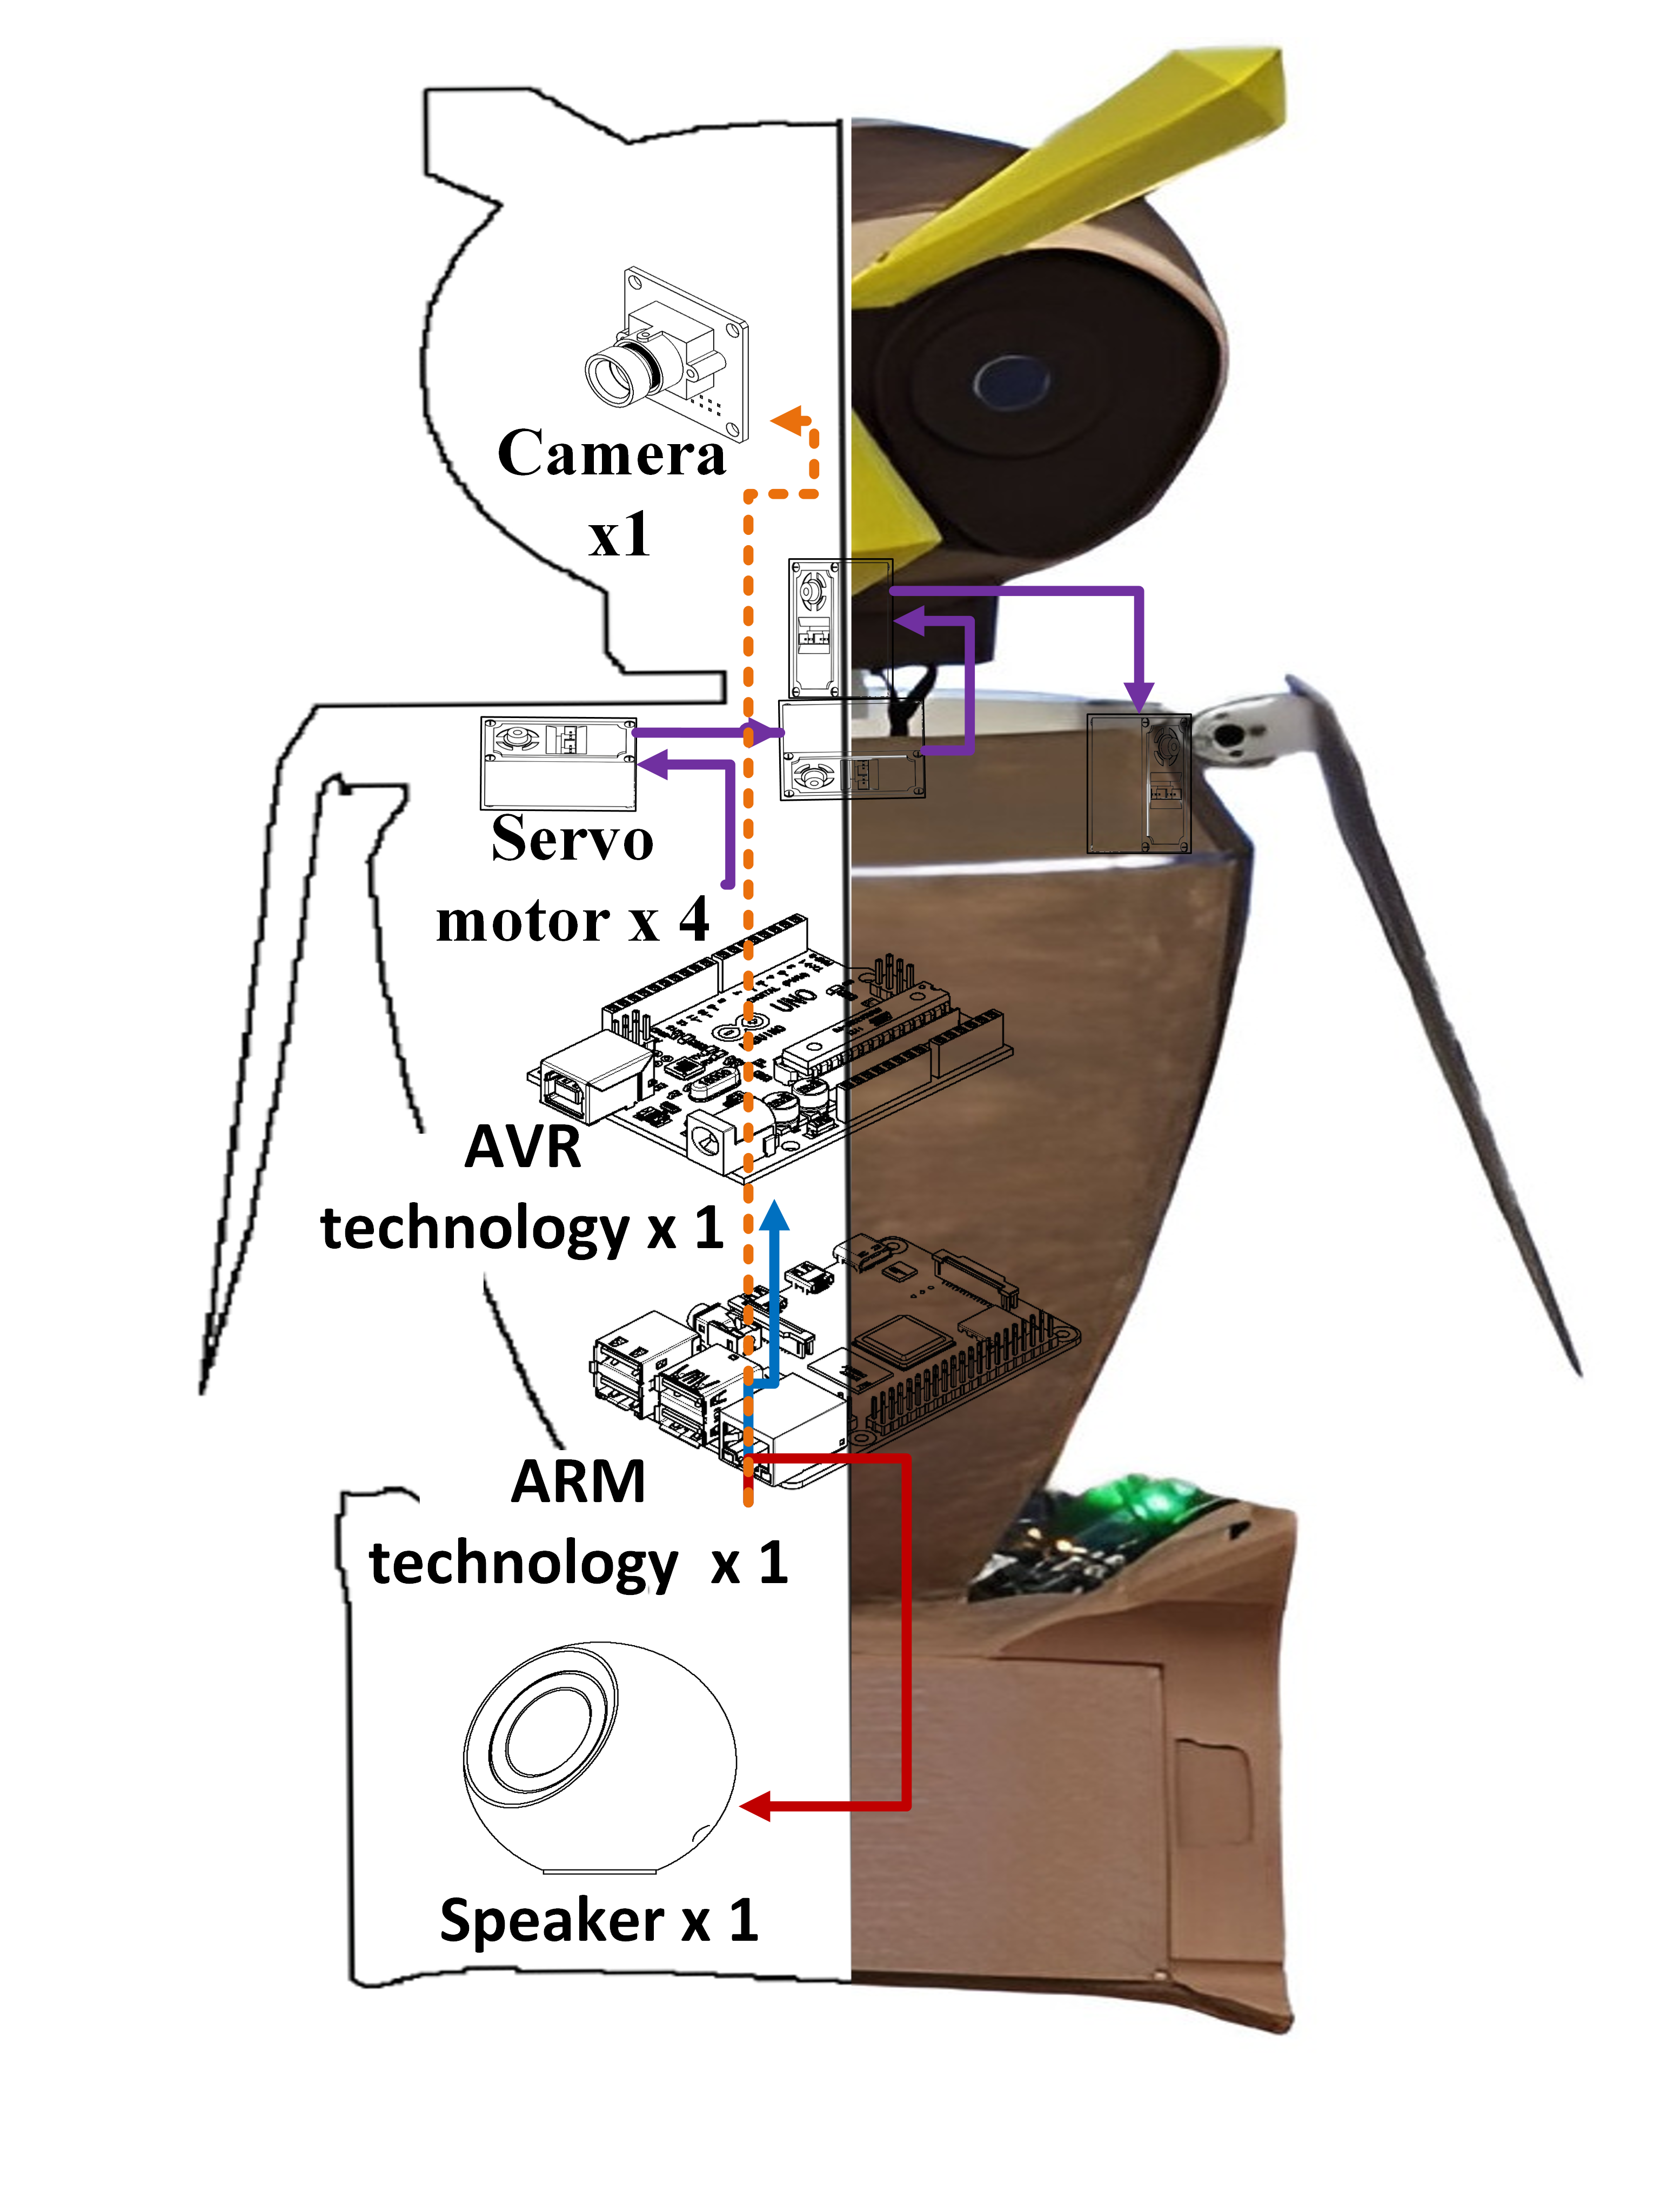
\includegraphics[width=\textwidth]{./images/Figure2.png}
		\caption{Structure and main components of the robotic assistant that represents an owl.}
		\label{Fig:Figure2}
		\source{Own work.}
\end{minipage}
\end{figure}



The system's operation begins with image capture through a camera embedded in one of the owl's eyes. These images are processed by the Raspberry Pi using a quantized classification model, optimized for low-power embedded devices. Based on the classification results, the Raspberry Pi generates specific commands that are transmitted to the Arduino to control the actuators. Additionally, the Raspberry Pi selects sounds corresponding to the detected categories during image processing and plays them in synchronization with the robot's movements, thereby enhancing the interactive experience.

Regarding the auditory feedback mechanism, the system utilizes a library of pre-recorded audio files stored locally on the Raspberry Pi. These sound clips were specifically selected to correspond semantically with the ten classes of the CIFAR-10 dataset; for instance, animal vocalizations were used for biological categories (e.g., a barking sound for the 'dog' class) and mechanical sound effects for transportation categories (e.g., an engine noise for the 'truck' class). The sounds were not generated synthetically in real-time; instead, they were sourced from open-access sound libraries and normalized for volume consistency. Upon classifying an image, the system retrieves the corresponding audio file and plays it immediately via the robot's speaker. This approach avoids the computational overhead and latency associated with real-time audio synthesis, ensuring the sound is perfectly synchronized with the robot's physical movements for effective reinforcement.

Motor control is managed by the Arduino, which operates the LX-15D servomotors. These servos enable precise movements in the owl's wings and head. Each wing possesses one degree of freedom, allowing vertical (up-and-down) motion. The head, in turn, has two degrees of freedom: horizontal rotation (left–right) and vertical tilt (up–down). In total, the system offers four degrees of freedom, distributed between the wings and the head, ensuring smooth and natural behavior. To this end, additive manufacturing was employed to construct each of the eight components that make up the robot. 

On the other hand, it is important to note that the Raspberry Pi 3 B+ microcomputer, on which the quantized neural network was implemented, is a recycled device. This model was released in March 2018 and features specifications\footnote{\url{https://www.raspberrypi.com/products/raspberry-pi-3-model-b-plus/}} that are now considered relatively limited:

\begin{itemize}
	\item Processor (CPU):
	\begin{itemize}
		\item Model: Broadcom BCM2837B0
		\item Architecture: 64-bit ARM Cortex-A53
		\item Cores: Quad-core
		\item Clock Speed: 1.4 GHz (an improvement over the 1.2 GHz of the Pi 3 B)
	\end{itemize}
	
	\item Memory (RAM):
	\begin{itemize}
		\item Capacity: 1 GB LPDDR2 SDRAM
	\end{itemize}
	
	\item Wireless Connectivity:
	\begin{itemize}
		\item Wi-Fi: Dual-band support (2.4 GHz and 5 GHz) compliant with IEEE 802.11.b/g/n/ac standards
		\item Bluetooth: Bluetooth 4.2 BLE (Bluetooth Low Energy)
		\item Antenna: Enhanced PCB antenna for improved wireless performance
	\end{itemize}
	
	\item Ethernet:
	\begin{itemize}
		\item Speed: Gigabit Ethernet port (up to 300 Mbps in real-world conditions, limited by USB 2.0 bandwidth)
		\item Improvement over the Pi 3 B, which featured a 10/100 Mbps Ethernet port
	\end{itemize}
	
	\item USB Ports:
	\begin{itemize}
		\item Quantity: 4 USB 2.0 ports
	\end{itemize}
	
	\item Video Output:
	\begin{itemize}
		\item HDMI: One standard HDMI port (supports resolutions up to 1080p)
		\item Composite Video Output: Available via 4-pole connector (shared audio/composite video)
	\end{itemize}
\end{itemize}


Similarly, by utilizing a recycled microcomputer, the overall construction cost of the robot is substantially reduced, since other components—such as the Arduino Nano board, motors, and camera—can also be sourced from recycled materials. \Cref{Tab:Table0} presents a list of the various components used in the robot's construction, as well as the additive manufacturing time required for each.


\begin{table}[h!]
\centering
\begin{threeparttable}
	\caption{List of components used for the fabrication of the robotic assistant through additive manufacturing; finishing elements (such as paint and similar materials) are not included.}
	\label{Tab:Table0}
	\begin{tabular}{lccc}
		\toprule
		Component & Unit Cost (USD) & Quantity & Subtotal (USD) \\
		\midrule
		Webcam & 14 & 1 & 14 \\
		Raspberry Pi 3 B+ & 45 & 1 & 45 \\
		Arduino Nano & 9 & 1 & 9 \\
		Additive manufacturing & 3.50 & 10 & 35 \\
		Servomotors LX-15D & 17 & 4 & 68 \\ 
		& &  Total & 171 \\
        \bottomrule
	\end{tabular}
	\source{Own work.}
	%\notes{Se necessário, poderá ser adicionada uma nota ao final da tabela.}	
\end{threeparttable}
\end{table}


\section{Pilot experiment and preliminary results}

\Cref{Fig:Figure3.1} illustrates the protocol followed to conduct the interaction process between the robotic assistant and the children. For the activity, ten pictograms from each category were printed, allowing the children to perform interaction exercises with the robot (ten images per category). During the interaction process, the classroom teacher was always present and responsible for instructing each child to place a specific pictogram. Additionally, two engineers participated in the session; they were responsible for providing technical support with the use of the robot, as well as documenting the entire interaction process and monitoring system performance (e.g., CPU usage, memory consumption, accuracy and error rates, among others).


\begin{figure}[h!]
\centering
\begin{minipage}{0.9\textwidth}
		%\includegraphics[width=\textwidth]{./images/Figure3.png}
		\centering
		\scalebox{0.8}{
		\begin{tikzpicture}[
			node distance=1.3cm and 2.8cm,
			font=\small,
			block/.style={draw, rounded corners=6pt, minimum width=3cm, minimum height=1.2cm, align=center},
			mynode/.style={draw, thick, rounded corners=8pt, fill=#1, inner sep=10pt},
			arrow/.style={thick, -{Stealth[]}}
			]
			
			% Central nodes
			\node[mynode=green!20] (pictos) {\begin{tabular}{c}\textbf{Pictogram Set}\\(10 Categories)\\\includegraphics[width=0.8cm]{images/pictograms.png}\end{tabular}};
			\node[mynode=blue!20, below=of pictos] (children) {\begin{tabular}{c}\textbf{Children}\\\includegraphics[width=0.8cm]{images/children.png}\end{tabular}};
			\node[mynode=orange!30, below=of children] (board) {\begin{tabular}{c}\textbf{Small Board}\\\includegraphics[width=0.7cm]{images/board.png}\end{tabular}};
			\node[mynode=cyan!30, below=of board] (webcam) {\begin{tabular}{c}\textbf{Webcam}\\\includegraphics[width=0.7cm]{images/webcam.png}\end{tabular}};
			
			% Side elements
			\node[mynode=pink!30, left=of children] (teacher) {\begin{tabular}{c}\textbf{Teacher}\\\includegraphics[width=0.8cm]{images/teacher.png}\end{tabular}};
			\node[mynode=red!20, right=of board] (owl) {\begin{tabular}{c}\textbf{Robotic Owl}\\\includegraphics[width=0.8cm]{images/owl.png}\end{tabular}};
			\node[mynode=yellow!30, above=of owl] (eng1) {\begin{tabular}{c}\textbf{Engineer 1}\\\includegraphics[width=0.8cm]{images/engineer.png}\end{tabular}};
			\node[mynode=yellow!30, below=of owl] (eng2) {\begin{tabular}{c}\textbf{Engineer 2}\\\includegraphics[width=0.8cm]{images/engineer.png}\end{tabular}};
			
			% Arrows
			\draw[arrow] (pictos) -- (children);
			\draw[arrow] (teacher.east) -- (children.west) node[midway, above] {Gives Command};
			\draw[arrow] (children) -- (board) node[midway, right] {Places Pictogram};
			\draw[arrow] (board) -- (webcam) node[midway, left] {Captured Image};
			
			% Frame capture label (2 lines)
			\draw[arrow] (webcam.east) to[bend left=15] (owl.south);
			\node at ($(webcam.east)!0.5!(owl.south) + (0,-0.5)$) {\begin{tabular}{c}Frames\\capture\end{tabular}};
			
			% Auditory Feedback: moved 0.8cm lower
			\draw[arrow] (owl.west) -- (children.east);
			\node at ($(owl.west)!0.5!(children.east) + (0,-0.9)$) {\begin{tabular}{c}Kinesthetic\\Feedback\end{tabular}};
			
			% Engineer arrows
			\draw[arrow] (eng1.south) -- node[midway, right] {System monitoring} (owl.north);
			\draw[arrow] (eng2.north) -- node[midway, right] {Registers interaction} (owl.south);
			
		\end{tikzpicture}
	}
		\caption{Diagram representing the interaction protocol involving children, a robotic owl, and supporting roles.}
		\label{Fig:Figure3.1}
		\source{Own work.}
\end{minipage}
\end{figure}


The classroom was prepared as follows. A desk was equipped with a small board on which the children placed the printed pictograms (see examples in Appendix \ref{app-i}). A webcam was positioned in front of the board to continuously capture video frames, which were sent to the robot for processing using the quantized neural network. The robot was placed next to the board in order to provide kinesthetic feedback to the children, indicating the recognized category.

Each time the teacher gave a command, the child was expected to place the corresponding pictogram on the board and receive immediate feedback indicating whether the selection was correct or incorrect (see Appendix \ref{app-ii}).

It is important to emphasize that this stage of the experimental process aimed to evaluate the children’s perception of the robot and to measure the accuracy of the system, as well as its capacity to operate continuously for several hours in a real-world environment (specifically, within the classroom of the ``Eugenio Espejo'' Educational Unit).

The following section presents the perception results obtained and the classification accuracy achieved by the neural network when recognizing the pictograms.

\subsection{Ethical Considerations}
The experimental protocol and interaction activities involving human subjects were reviewed and authorized by the institutional authorities of the ``Unidad Educativa Eugenio Espejo'' (Institutional Review Board). Formal approval was granted by the Director of the institution, ensuring compliance with educational and ethical standards for working with minors.

Prior to the study, informed consent was obtained from the school administration and the parents or legal guardians of all participating children. The study was conducted in the presence of the classroom teacher to ensure a safe and familiar environment. No personally identifiable information (PII) beyond age and gender was stored; all video data processed by the robot was analyzed in real-time and not permanently recorded, preserving the privacy and anonymity of the participants.

\subsection{Perception analysis of the robotic assistant: a pilot study involving 52 children}

With the aim of determining how users perceive the tool, a survey was administered to two groups of children enrolled in the second and third years of General Basic Education (GBE) at the ``Eugenio Espejo'' Educational Unit. A total of 52 children participated in the study, with their ages and grade levels detailed in \Cref{Tab:Table1}.


\begin{table}[h!]
\centering
\begin{threeparttable}
	\caption{Distribution of surveyed children according to their grade level in basic education and their age.}
	\label{Tab:Table1}
	\begin{tabular}{ccc}
		\toprule
		Grade Level & Age & Total \\
		\midrule
		Second Grade & 5 & 3 \\ 
		Second Grade & 6 & 21 \\ 		
		Second Grade & 8 & 1 \\ 
		Third Grade & 6 & 1 \\ 
		Third Grade & 7 & 21 \\ 
		Third Grade & 8 & 5 \\ 
		&  Total & 52 \\ 
        \bottomrule
	\end{tabular}
	\source{Own work.}
	%\notes{Se necessário, poderá ser adicionada uma nota ao final da tabela.}	
\end{threeparttable}
\end{table}


As shown in \Cref{Tab:Table1}, there are 25 children enrolled in the second year of GBE and 27 children in the third year. The age range spans from 6 to 8 years, with a mean age of 5.96 and a standard deviation (SD) of 0.539 for the second-year group, and a mean of 7.15 with an SD of 0.456 for the third-year group.

It is important to note the presence of outliers, such as the three 5-year-old children and the 8-year-old child enrolled in the second year (\Cref{Fig:Figure3}). 

Similarly, five children aged 8 are enrolled in the third year of GBE. This situation may be attributed to various factors, such as children having started earlier in previous educational levels or having experienced health-related delays that postponed their school entry.


\begin{figure}[h!]
\centering
\begin{minipage}{.83\textwidth}
		\includegraphics[width=\textwidth]{./images/Figure3.png}
		\caption{Box-and-whisker plot of the age distribution of the surveyed children, disaggregated by gender.}
		\label{Fig:Figure3}
		\source{Own work.}
\end{minipage}
\end{figure}



The survey is composed of two sections: three demographic questions (age, gender, and current grade level in basic education) and thirteen items using a Likert scale. The questions in the second section focus on assessing the following aspects (with the corresponding question numbers as shown in Figures \ref{Fig:Figure4} and \ref{Fig:Figure5}):

\begin{itemize}
	\item Perception of the owl's physical characteristics: shape (Q01), size (Q02), colors (Q03), movements (Q04), and the voice used to provide feedback to the user (Q05).
	
	\item Perception of the content of the pictograms used: modes of transportation (Q06), domestic animals (Q07), and wild animals (Q08).
	
	\item Perception of the size of the images (Q09), and the perceived usefulness of having the robotic assistant in the classroom (Q10) or at home (Q11).
	
	\item Perception of the robotic assistant's ability to recognize pictograms (Q12) and to display them on screen (Q13).
	
\end{itemize}


To validate the survey, \posscite{bujang2018review} coefficient was employed, yielding a value of 0.71, which indicates an ``acceptable'' level of internal consistency among the items. This result is considered satisfactory given that the instrument is newly developed and takes into account the inherent challenges of working with children aged 6 to 8 years.


As shown in \Cref{Fig:Figure4}, 19.2\% of the children indicated that they ``like'' the shape of the robot (Q01), while 73.1\% reported that they ``like it very much.'' Regarding the size of the owl (Q02), the children's perceptions were distributed as follows: ``normal'' (30.8\%), ``large'' (19.2\%), and ``very large'' (48.1\%). The colors of the robot (Q03) were perceived as ``very nice'' (69.2\%) and ``nice'' (25\%). The robot's movements (Q04) were perceived as ``very nice'' (51.9\%), ``nice'' (26.9\%), and ``neither nice nor unpleasant'' (11.5\%). The robot's voice (Q05) was primarily described as ``very nice'' (61.5\%) and ``nice'' (25\%).

Similarly, the pictograms representing means of transportation (Q06), domestic animals (Q07), and wild animals (Q08) were perceived as ``very nice'' and ``nice,'' with percentages of 65.4\% and 19.2\%, 67\% and 28.8\%, and 69.2\% and 21.2\%, respectively.

Furthermore, the mean Likert scale scores for these questions all exceeded 4, indicating that the majority of respondents expressed a highly positive perception regarding the aforementioned criteria.

\begin{figure}[h!]
	\centering
	\begin{minipage}{.9\textwidth}
		\includegraphics[width=\textwidth]{./images/Figure4.png}
		\caption{Children's perceptions regarding the first eight questions of the survey, which relate to the physical characteristics of the robot and the pictograms depicting means of transportation, domestic animals, and wild animals.}
		\label{Fig:Figure4}
		\source{Own work.}
	\end{minipage}
\end{figure}

\Cref{Fig:Figure5} presents the results corresponding to the remaining set of survey questions. Regarding the size of the images (Q09), most children perceived them as either ``very large'' (40.4\%¸) or ``normal'' (38.5\%¸). A majority of respondents ``strongly agreed'' with the idea of having the owl robot at home (Q10) and at school (Q11) to support learning about means of transportation and animals, with percentages of 73.1\%¸ and 67.3\%¸, respectively.

Moreover, children reported that they ``liked very much'' (67.3\%¸) or ``liked'' (21.2\%¸) the way the robot recognizes images (Q12) through the neural network. As for the way in which the images are displayed on the screen (Q13), perceptions were similarly positive, with responses primarily distributed between ``liked very much'' (69.2\%¸) and ``liked'' (23.1\%¸). As observed in the group of questions described in \Cref{Fig:Figure5}, all items received a mean score above 4 on the Likert scale, with the exception of question Q09.

\begin{figure}[h!]
	\centering
	\begin{minipage}{.9\textwidth}
		\includegraphics[width=\textwidth]{./images/Figure5.png}
		\caption{Children's perceptions regarding the final five questions of the survey, which relate to the size of the images, the possibility of having the robot at home, and the way in which the robot recognizes images through the neural network.}
		\label{Fig:Figure5}
		\source{Own work.}
	\end{minipage}
\end{figure}


\subsection{Accuracy of the quantized neural network: category-wise confusion analysis}

In order to assess the accuracy with which the quantized neural network classifies images by category, a confusion matrix was computed, as illustrated in \Cref{Fig:FigureG}. As observed, the values along the diagonal represent the number of correctly classified images for each class, whereas the off-diagonal values correspond to images that were misclassified into other categories (indicated on both the $X$ and $Y$ axes).

The matrix reveals that the model achieves relatively high accuracy in classes such as ``automobile'' and ``truck'', while it encounters greater difficulty with classes such as ``cat'' and ``ship'', which exhibit a higher number of misclassifications. This suggests that although the model performs well in certain categories, further improvement is needed in distinguishing between specific classes.

\begin{figure}[h!]
	\centering
	\begin{minipage}{.7\textwidth}
		\includegraphics[width=\textwidth]{./images/FigureG.png}
		\caption{Confusion matrix illustrating the classification results on the test set. It highlights the image categories that are misclassified by the quantized neural network.}
		\label{Fig:FigureG}
		\source{Own work.}
	\end{minipage}
\end{figure}



\section{Conclusions}

The study show that dynamic quantization is an effective strategy for optimizing deep neural networks, enabling their deployment on low-resource embedded systems without significant loss in performance. By integrating a quantized MobileNetV3 Small model into an owl-shaped interactive robotic assistant, the research provides a practical and low-cost solution for educational environments, particularly in contexts with limited technological infrastructure. 

The pilot carried out with children aged 5 to 8 years showed a high level of acceptance and positive perception toward both the robot and its functionalities, including pictogram recognition and visual feedback. These findings highlight the potential of the proposed system as a valuable tool for supporting cognitive development and enhancing learning experiences through playful, human-robot interaction.

The following future work lines are proposed:

\begin{itemize}
	\item Conduct a second training phase of the neural network to enable it to recognize real objects.
	
	\item Develop a text-to-speech module to provide instructions or commands to children, employing Spanish with an Ecuadorian accent.
	
	\item Integrate a computer vision system with two cameras to allow the robot to perceive the distance of objects.
\end{itemize}





%\printbibliography\label{sec-bib}

% if the text is not in Portuguese, it might be necessary to use the code below instead to print the correct ABNT abbreviations [s.n.], [s.l.]

%\begin{portuguese}
%\printbibliography[title={Bibliography}]
%\end{portuguese}


\printbibliography




%full list: conceptualization,datacuration,formalanalysis,funding,investigation,methodology,projadm,resources,software,supervision,validation,visualization,writing,review

\begin{contributors}[sec-contributors]
\authorcontribution{Lisseth Padilla-Vi{\~n}anzaca}[investigation, methodology, software, validation, writing]
\authorcontribution{Bryam Guach{\'u}n-Guam{\'a}n}[investigation, methodology, software, validation, writing]
\authorcontribution{Vladimir Robles-Bykbaev}[conceptualization, datacuration, formalanalysis, methodology, writing,review]
\authorcontribution{Efrén Lema-Condo}[investigation, methodology, writing]

\end{contributors}

\begin{dataavailability}
\txtdataavailability{dataavailable} % options: dataavailable, dataonly, databody, datanotav, nodata
\end{dataavailability}

\appendix 
\section{Appendix I}\label{app-i}

Figure \ref{Fig:Figureai} presents three photographs documenting the interaction process with the children. The top photograph shows a girl placing pictograms on the small board so that the webcam can recognize the image category. In the bottom-left photograph, a group of children can be seen becoming familiar with the activity while the teacher and engineers provide guidance on how to correctly position the pictograms for the recognition process. The bottom-right photograph captures the moment when the children receive feedback from the robotic assistant, delivered through auditory cues and movements of the owl’s wings and head.

\begin{figure}[h!]
	\centering
	\begin{minipage}{.7\textwidth}
		\includegraphics[width=\textwidth]{./images/Appendixi.png}
		\caption{Photographs taken during the interaction process between the children and the robotic assistant. The activity was conducted in a classroom at the ``Eugenio Espejo'' Educational Unit.}
		\label{Fig:Figureai}
		\source{Own work.}
	\end{minipage}
\end{figure}


%\appendix 
\section{Appendix II}\label{app-ii}

\Cref{Fig:Figureaii} presents four examples of pictograms that were printed for the interaction process with the children. As shown, the pictograms represent the following categories: horses (top left), frogs (top right), airplanes (bottom left), and dogs (bottom right). It is important to note that these images were obtained from the Pexels website (\url{https://www.pexels.com/}) and were not used during the training phase of the neural network.

\begin{figure}[h!]
	\centering
	\begin{minipage}{.7\textwidth}
		\includegraphics[width=\textwidth]{./images/Appendixii.png}
		\caption{Example images that were printed for the interaction activity with the children. The images were scaled to fit within an A4-sized sheet.}
		\label{Fig:Figureaii}
		\source{Pexels (horse: Helena Lopes - \url{https://www.pexels.com/photo/white-horse-running-on-green-field-1996337/} , frog: Susanne Jutzeler - \url{https://www.pexels.com/photo/a-frog-sitting-on-a-rock-in-front-of-water-27098494/}, airplain: Pascal Borener - \url{https://www.pexels.com/photo/white-and-yellow-tigerair-airplane-105821/}, and dog: Alexas Fotos - \url{https://www.pexels.com/photo/close-up-shot-of-a-dog-12800442/}.)}
	\end{minipage}
\end{figure}


\end{document}

